% Options for packages loaded elsewhere
% Options for packages loaded elsewhere
\PassOptionsToPackage{unicode}{hyperref}
\PassOptionsToPackage{hyphens}{url}
%
\documentclass[
  english,
  russian,
  12pt,
  a4paper,
  DIV=11,
  numbers=noendperiod]{scrreprt}
\usepackage{xcolor}
\usepackage{amsmath,amssymb}
\setcounter{secnumdepth}{5}
\usepackage{iftex}
\ifPDFTeX
  \usepackage[T1]{fontenc}
  \usepackage[utf8]{inputenc}
  \usepackage{textcomp} % provide euro and other symbols
\else % if luatex or xetex
  \usepackage{unicode-math} % this also loads fontspec
  \defaultfontfeatures{Scale=MatchLowercase}
  \defaultfontfeatures[\rmfamily]{Ligatures=TeX,Scale=1}
\fi
\usepackage{lmodern}
\ifPDFTeX\else
  % xetex/luatex font selection
\fi
% Use upquote if available, for straight quotes in verbatim environments
\IfFileExists{upquote.sty}{\usepackage{upquote}}{}
\IfFileExists{microtype.sty}{% use microtype if available
  \usepackage[]{microtype}
  \UseMicrotypeSet[protrusion]{basicmath} % disable protrusion for tt fonts
}{}
\usepackage{setspace}
% Make \paragraph and \subparagraph free-standing
\makeatletter
\ifx\paragraph\undefined\else
  \let\oldparagraph\paragraph
  \renewcommand{\paragraph}{
    \@ifstar
      \xxxParagraphStar
      \xxxParagraphNoStar
  }
  \newcommand{\xxxParagraphStar}[1]{\oldparagraph*{#1}\mbox{}}
  \newcommand{\xxxParagraphNoStar}[1]{\oldparagraph{#1}\mbox{}}
\fi
\ifx\subparagraph\undefined\else
  \let\oldsubparagraph\subparagraph
  \renewcommand{\subparagraph}{
    \@ifstar
      \xxxSubParagraphStar
      \xxxSubParagraphNoStar
  }
  \newcommand{\xxxSubParagraphStar}[1]{\oldsubparagraph*{#1}\mbox{}}
  \newcommand{\xxxSubParagraphNoStar}[1]{\oldsubparagraph{#1}\mbox{}}
\fi
\makeatother


\usepackage{longtable,booktabs,array}
\newcounter{none} % for unnumbered tables
\usepackage{calc} % for calculating minipage widths
% Correct order of tables after \paragraph or \subparagraph
\usepackage{etoolbox}
\makeatletter
\patchcmd\longtable{\par}{\if@noskipsec\mbox{}\fi\par}{}{}
\makeatother
% Allow footnotes in longtable head/foot
\IfFileExists{footnotehyper.sty}{\usepackage{footnotehyper}}{\usepackage{footnote}}
\makesavenoteenv{longtable}
\usepackage{graphicx}
\makeatletter
\newsavebox\pandoc@box
\newcommand*\pandocbounded[1]{% scales image to fit in text height/width
  \sbox\pandoc@box{#1}%
  \Gscale@div\@tempa{\textheight}{\dimexpr\ht\pandoc@box+\dp\pandoc@box\relax}%
  \Gscale@div\@tempb{\linewidth}{\wd\pandoc@box}%
  \ifdim\@tempb\p@<\@tempa\p@\let\@tempa\@tempb\fi% select the smaller of both
  \ifdim\@tempa\p@<\p@\scalebox{\@tempa}{\usebox\pandoc@box}%
  \else\usebox{\pandoc@box}%
  \fi%
}
% Set default figure placement to htbp
\def\fps@figure{htbp}
\makeatother



\ifLuaTeX
\usepackage[bidi=basic,shorthands=off,provide=*]{babel}
\else
\usepackage[bidi=default,shorthands=off,provide=*]{babel}
\fi
\ifLuaTeX
  \usepackage{selnolig} % disable illegal ligatures
\fi


\setlength{\emergencystretch}{3em} % prevent overfull lines

\providecommand{\tightlist}{%
  \setlength{\itemsep}{0pt}\setlength{\parskip}{0pt}}



 
\usepackage[style=gost-numeric,backend=biber,langhook=extras,autolang=other*]{biblatex}
\addbibresource{bib/cite.bib}

\usepackage[]{csquotes}

\usepackage{indentfirst}
\usepackage{float}
\floatplacement{figure}{H}
\IfFileExists{plex-otf.sty}{
  %% Full TeXlive
  \usepackage[
    % math,
    RM={Scale=0.94},SS={Scale=0.94},SScon={Scale=0.94},TT={Scale=MatchLowercase,FakeStretch=0.9},
    DefaultFeatures={Ligatures=Common}
  ]{plex-otf}
  % \usepackage[Scale=MatchUppercase]{juliamono}
}{
  %% TinyTeX
  \usepackage{libertine}
}
\KOMAoption{captions}{tableheading}
\makeatletter
\@ifpackageloaded{caption}{}{\usepackage{caption}}
\AtBeginDocument{%
\ifdefined\contentsname
  \renewcommand*\contentsname{Содержание}
\else
  \newcommand\contentsname{Содержание}
\fi
\ifdefined\listfigurename
  \renewcommand*\listfigurename{Список иллюстраций}
\else
  \newcommand\listfigurename{Список иллюстраций}
\fi
\ifdefined\listtablename
  \renewcommand*\listtablename{Список таблиц}
\else
  \newcommand\listtablename{Список таблиц}
\fi
\ifdefined\figurename
  \renewcommand*\figurename{Рисунок}
\else
  \newcommand\figurename{Рисунок}
\fi
\ifdefined\tablename
  \renewcommand*\tablename{Таблица}
\else
  \newcommand\tablename{Таблица}
\fi
}
\@ifpackageloaded{float}{}{\usepackage{float}}
\floatstyle{ruled}
\@ifundefined{c@chapter}{\newfloat{codelisting}{h}{lop}}{\newfloat{codelisting}{h}{lop}[chapter]}
\floatname{codelisting}{Список}
\newcommand*\listoflistings{\listof{codelisting}{Листинги}}
\makeatother
\makeatletter
\makeatother
\makeatletter
\@ifpackageloaded{caption}{}{\usepackage{caption}}
\@ifpackageloaded{subcaption}{}{\usepackage{subcaption}}
\makeatother
\usepackage{bookmark}
\IfFileExists{xurl.sty}{\usepackage{xurl}}{} % add URL line breaks if available
\urlstyle{same}
\hypersetup{
  pdftitle={Шаблон отчёта по лабораторной работе},
  pdfauthor={Дмитрий Сергеевич Кулябов},
  pdflang={ru-RU},
  pdfkeywords={лабораторная работа, шаблон, Markdown, Pandoc},
  hidelinks,
  pdfcreator={LaTeX via pandoc}}


\title{Шаблон отчёта по лабораторной работе}
\usepackage{etoolbox}
\makeatletter
\providecommand{\subtitle}[1]{% add subtitle to \maketitle
  \apptocmd{\@title}{\par {\large #1 \par}}{}{}
}
\makeatother
\subtitle{Простейший вариант}
\author{Дмитрий Сергеевич Кулябов}
\date{}
\begin{document}
\maketitle
\begin{abstract}
В данном отчёте представлены результаты выполнения лабораторной работы
по теме \ldots{}

Описаны использованные методы, полученные экспериментальные данные и их
анализ.

Сделаны выводы о достижении поставленной цели.
\end{abstract}

\renewcommand*\contentsname{Содержание}
{
\setcounter{tocdepth}{1}
\tableofcontents
}
\listoffigures
\listoftables

\setstretch{1.5}
\chapter{Введение}\label{ux432ux432ux435ux434ux435ux43dux438ux435}

\section{Актуальность}\label{ux430ux43aux442ux443ux430ux43bux44cux43dux43eux441ux442ux44c}

Здесь обосновывается, почему данная работа важна, какое место она
занимает в курсе или в научной проблематике.

\section{Цель
работы}\label{ux446ux435ux43bux44c-ux440ux430ux431ux43eux442ux44b}

Здесь приводится формулировка цели лабораторной работы. Формулировки
цели для каждой лабораторной работы приведены в методических указаниях.

Цель данного шаблона --- максимально упростить подготовку отчётов по
лабораторным работам. Модифицируя данный шаблон, студенты смогут без
труда подготовить отчёт по лабораторным работам, а также познакомиться с
основными возможностями разметки Markdown.

\section{Задачи}\label{ux437ux430ux434ux430ux447ux438}

Перечисляются конкретные шаги, которые необходимо выполнить для
достижения цели.

\section{Объект и предмет
исследования}\label{ux43eux431ux44aux435ux43aux442-ux438-ux43fux440ux435ux434ux43cux435ux442-ux438ux441ux441ux43bux435ux434ux43eux432ux430ux43dux438ux44f}

Кратко описывается, что исследуется и в каком аспекте.

\section{Методы
исследования}\label{ux43cux435ux442ux43eux434ux44b-ux438ux441ux441ux43bux435ux434ux43eux432ux430ux43dux438ux44f}

Указываются основные методы, используемые в работе (экспериментальные,
расчётные, моделирование и т.д.).

\section{Схема выполнения
работы}\label{ux441ux445ux435ux43cux430-ux432ux44bux43fux43eux43bux43dux435ux43dux438ux44f-ux440ux430ux431ux43eux442ux44b}

На рис. \ref{fig-flowchart} представлена общая последовательность
действий при выполнении работы.

\begin{figure}

\centering{

\pandocbounded{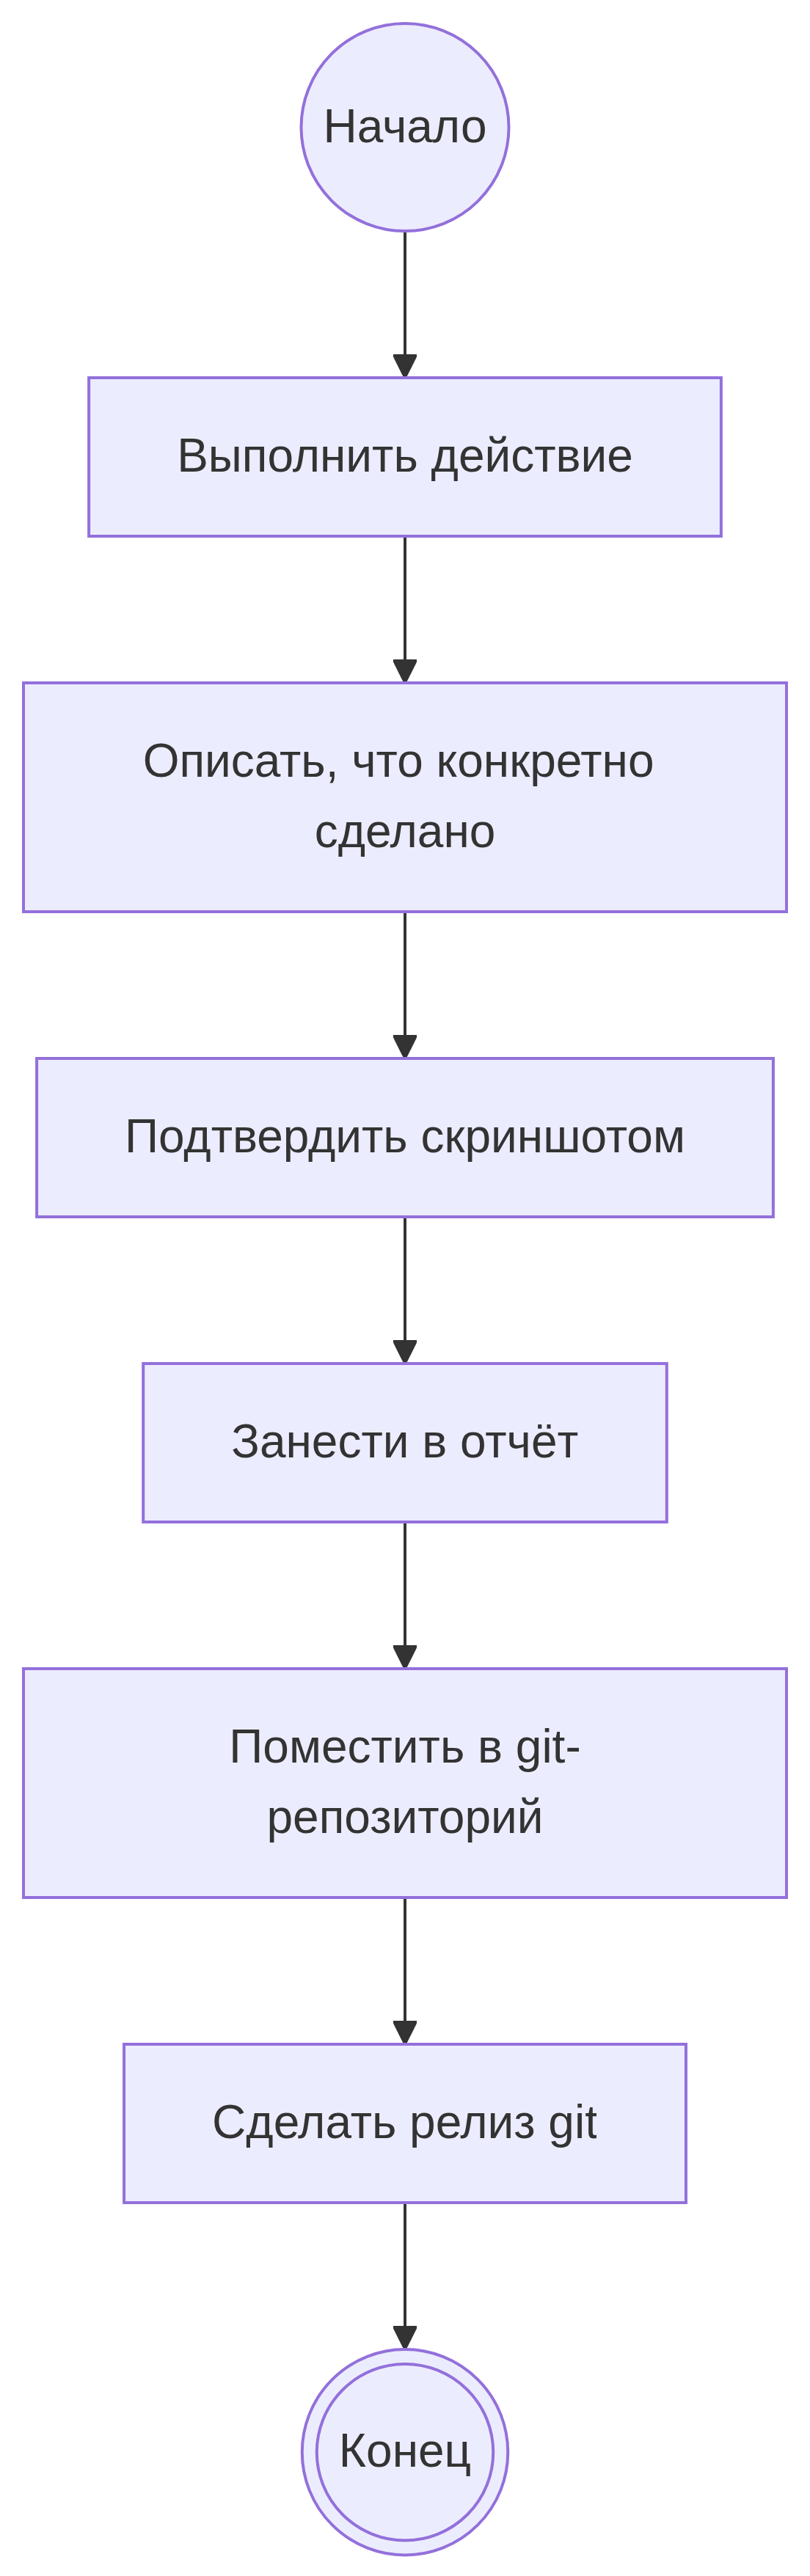
\includegraphics[keepaspectratio]{os-intro-lab01-os-intro-lab01-report_files/figure-latex/mermaid-figure-2.png}}

}

\caption{\label{fig-flowchart}Блок-схема выполнения лабораторной работы}

\end{figure}%

\chapter{Теоретическая
часть}\label{ux442ux435ux43eux440ux435ux442ux438ux447ux435ux441ux43aux430ux44f-ux447ux430ux441ux442ux44c}

Здесь излагаются теоретические сведения, необходимые для понимания
работы. Это может быть описание файловой системы, алгоритмов, физических
законов и т.п.

Например, в табл. \ref{tbl-std-dir} приведено краткое описание
стандартных каталогов Unix.

\begin{longtable}[]{@{}
  >{\raggedright\arraybackslash}p{(\linewidth - 2\tabcolsep) * \real{0.1014}}
  >{\raggedright\arraybackslash}p{(\linewidth - 2\tabcolsep) * \real{0.8986}}@{}}
\caption{Описание некоторых каталогов файловой системы GNU
Linux}\label{tbl-std-dir}\tabularnewline
\toprule\noalign{}
\begin{minipage}[b]{\linewidth}\raggedright
Имя каталога
\end{minipage} & \begin{minipage}[b]{\linewidth}\raggedright
Описание каталога
\end{minipage} \\
\midrule\noalign{}
\endfirsthead
\toprule\noalign{}
\begin{minipage}[b]{\linewidth}\raggedright
Имя каталога
\end{minipage} & \begin{minipage}[b]{\linewidth}\raggedright
Описание каталога
\end{minipage} \\
\midrule\noalign{}
\endhead
\bottomrule\noalign{}
\endlastfoot
\texttt{/} & Корневая директория, содержащая всю файловую систему \\
\texttt{/bin} & Основные системные утилиты, необходимые как в
однопользовательском режиме, так и при обычной работе всем
пользователям \\
\texttt{/etc} & Общесистемные конфигурационные файлы и файлы
конфигурации установленных программ \\
\texttt{/home} & Содержит домашние директории пользователей, которые, в
свою очередь, содержат персональные настройки и данные пользователя \\
\texttt{/media} & Точки монтирования для сменных носителей \\
\texttt{/root} & Домашняя директория пользователя \texttt{root} \\
\texttt{/tmp} & Временные файлы \\
\texttt{/usr} & Вторичная иерархия для данных пользователя \\
\end{longtable}

Более подробно про Unix см. в
\autocite{tanenbaum_book_modern-os_ru,robbins_book_bash_en,zarrelli_book_mastering-bash_en,newham_book_learning-bash_en}.

\chapter{Материалы и
методы}\label{ux43cux430ux442ux435ux440ux438ux430ux43bux44b-ux438-ux43cux435ux442ux43eux434ux44b}

В этом разделе описывается, как именно выполнялась работа:

\begin{itemize}
\tightlist
\item
  оборудование, программное обеспечение, реактивы;
\item
  последовательность действий, настройки параметров;
\item
  методы сбора и обработки данных.
\end{itemize}

\chapter{Выполнение лабораторной
работы}\label{ux432ux44bux43fux43eux43bux43dux435ux43dux438ux435-ux43bux430ux431ux43eux440ux430ux442ux43eux440ux43dux43eux439-ux440ux430ux431ux43eux442ux44b}

Описываются проведённые действия.

Каждый шаг документируется скриншотом (рис. \ref{fig-001}).

\begin{figure}

\centering{

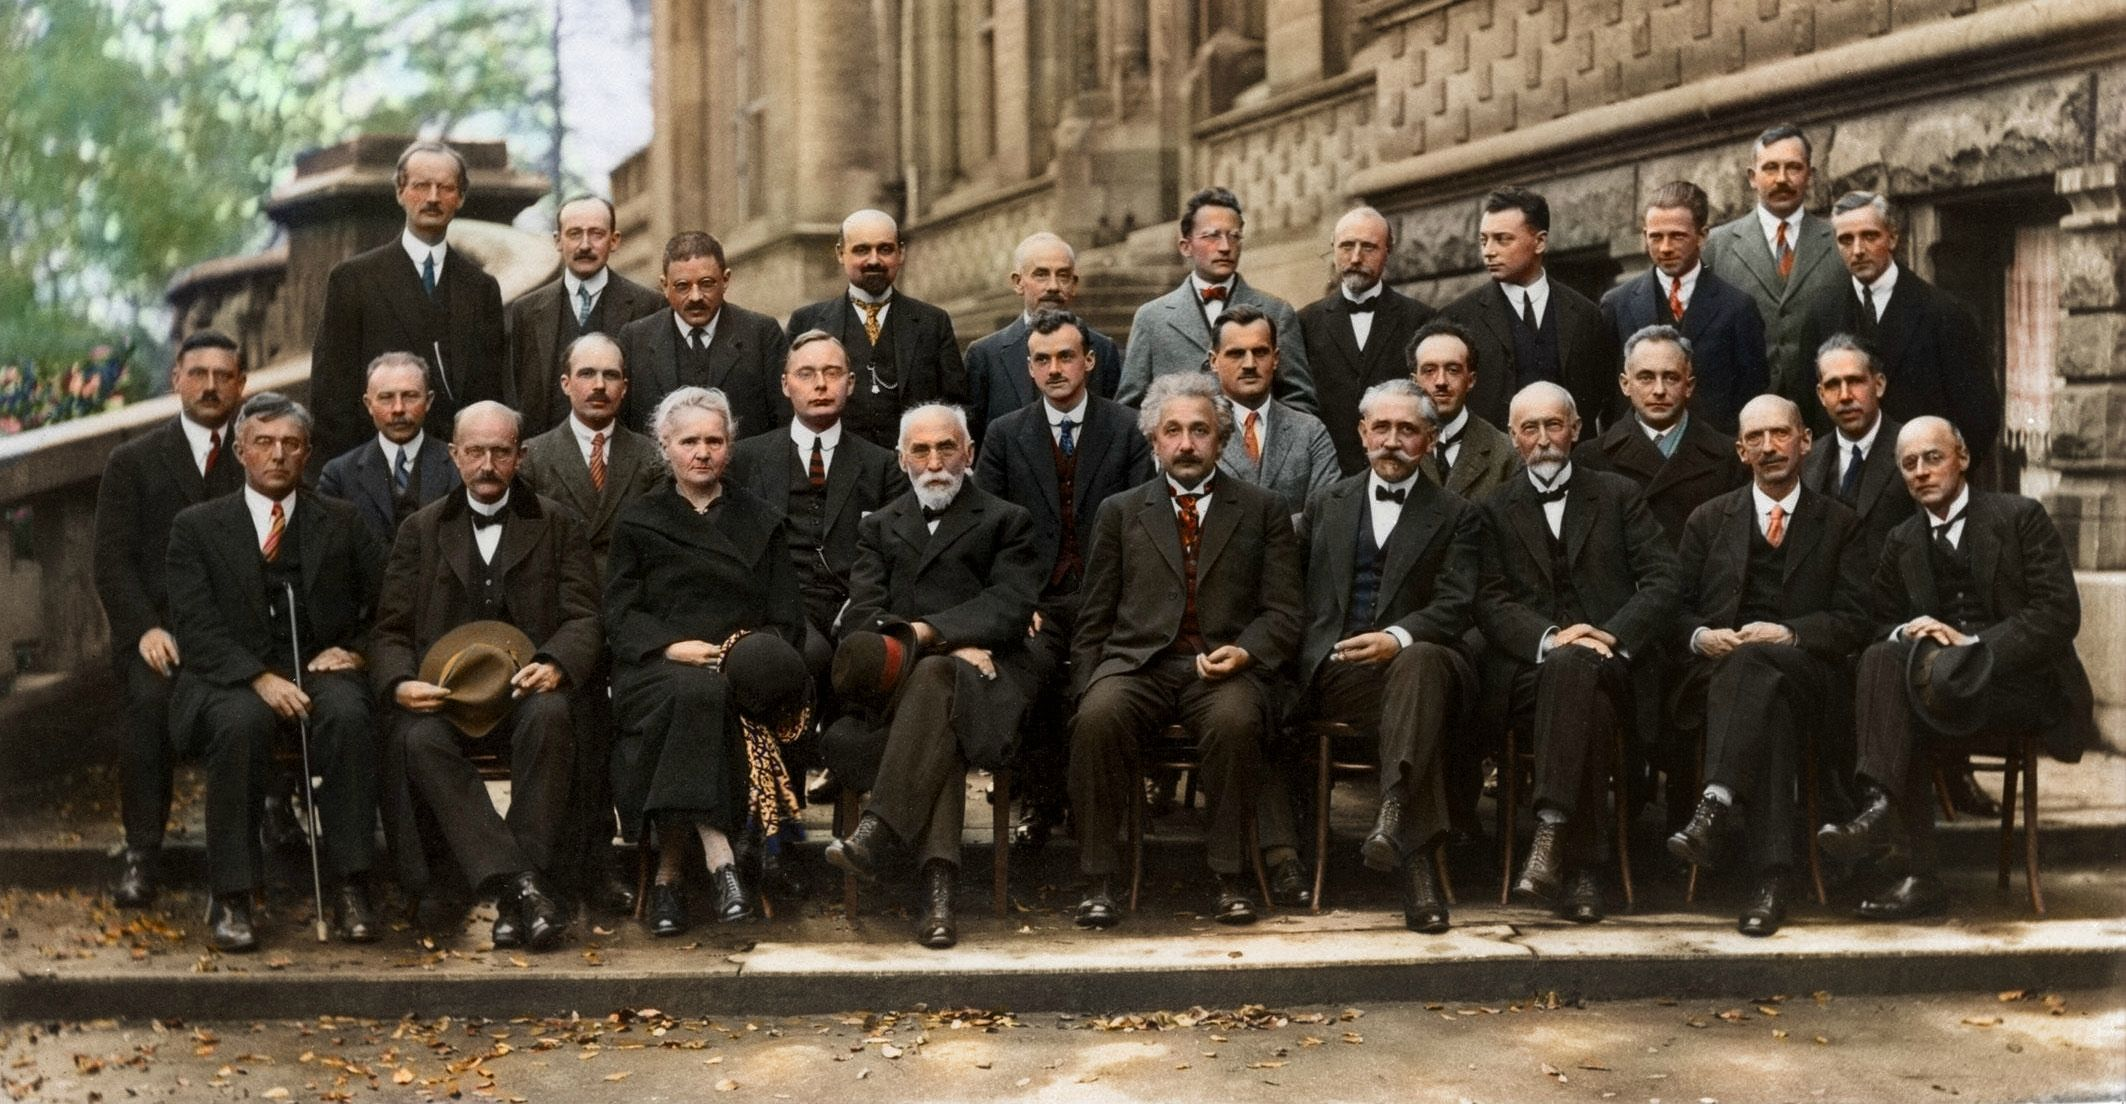
\includegraphics[width=0.7\linewidth,height=\textheight,keepaspectratio]{image/solvay.jpg}

}

\caption{\label{fig-001}V Сольвеевский конгресс (1927) «Электроны и
фотоны»}

\end{figure}%

Каждый скриншот должен иметь подпись. На каждый скриншот должна быть
ссылка.

\chapter{Результаты}\label{ux440ux435ux437ux443ux43bux44cux442ux430ux442ux44b}

Здесь приводятся объективные данные, полученные в ходе работы. Это могут
быть таблицы с измерениями, графики, выводы программ, скриншоты. Без
интерпретации --- только констатация фактов.

\chapter{Обсуждение
результатов}\label{ux43eux431ux441ux443ux436ux434ux435ux43dux438ux435-ux440ux435ux437ux443ux43bux44cux442ux430ux442ux43eux432}

В этом разделе проводится анализ полученных результатов:

\begin{itemize}
\tightlist
\item
  сопоставление с теоретическими ожиданиями;
\item
  сравнение с данными других авторов;
\item
  объяснение возможных отклонений, погрешностей;
\item
  практическая значимость результатов.
\end{itemize}

\chapter{Заключение}\label{ux437ux430ux43aux43bux44eux447ux435ux43dux438ux435}

Кратко, по пунктам, перечисляются главные итоги работы:

\begin{itemize}
\tightlist
\item
  Достигнута ли поставленная цель;
\item
  Какие конкретные результаты получены;
\item
  Рекомендации по применению или направления для дальнейших
  исследований.
\end{itemize}

\chapter*{Список
литературы}\label{ux441ux43fux438ux441ux43eux43a-ux43bux438ux442ux435ux440ux430ux442ux443ux440ux44b}
\addcontentsline{toc}{chapter}{Список литературы}

\printbibliography[heading=none]

\appendix

\chapter{Что выносится в
приложения}\label{ux447ux442ux43e-ux432ux44bux43dux43eux441ux438ux442ux441ux44f-ux432-ux43fux440ux438ux43bux43eux436ux435ux43dux438ux44f}

При необходимости сюда выносятся:

\begin{itemize}
\tightlist
\item
  листинги программ;
\item
  большие таблицы с исходными данными;
\item
  промежуточные выкладки;
\item
  акты внедрения и т.п.
\end{itemize}

Каждое приложение начинается с новой страницы и имеет заголовок
(например, «Приложение А. Листинг программы»).





\end{document}
